\chapter{Background}
\label{chap:background}

The readers benefit from an understanding regarding the state-of-the-art and the 
current challenges presented in the field of parallel computing and deep 
learning in order to grasp the works carried out from this thesis.
Section~\ref{sec:mps} prepares the reader with the acquaintances of the various 
forms of modern parallel systems. Section~\ref{sec:ppm} provides backgrounds on 
the parallel programming models on modern parallel systems. Subsequently, 
section~\ref{sec:solvers} and~\ref{sec:dnn} present an introduction to the two 
application domains this work deals with, namely, parallel numerical algorithms 
and DNNs.

\section{Modern Parallel Systems}
\label{sec:mps}
The Exascale supercomputers are expected to come into operation near 2020. In 
order to reach that, major improvements need to be achieved including the energy 
and power, memory and storage, concurrency and locality and 
resiliency~\cite{doe}. Nevertheless, the mainstream trend stays with the massive 
parallelism with accelerators approach. This section provides a background on 
both types of systems and an introduction to some major parallel programming 
models.

With the roll-out of 7 and 5 nm node, the VLSI (very large scale integration) 
manufacturing technology is rapidly approaching its end due to its physical 
limitation. Furthermore, the power and energy consumption, as a consequence the 
heat dissipation, on a modern VLSI chip has become a major limiting factor in 
processor design. All the above impede the efforts to push a single-core 
processor to go faster. In response, industry turns its attention into designing 
multi-core multiprocessor systems which exploit parallelism at the application 
level. Figure~\ref{fig:multicore} illustrates a typical multi-core 
multiprocessor system~\cite{ibm_multicore}. Each of the processor (processor 0 
and 1) packs two separate cores with their own L1 and L2 cache. The two 
processors are connected via a system bus which also connects to the RAM. All 
the cores thus are able to access to the entire memory region. Nonetheless, 
since all the access to the memory and communication among processors are 
conducted on the system bus, the system is limited in its scale in that the 
inevitable contention on the bus system while the number of processors grows 
eventually renders a large-scale system unresponsive.
\begin{figure}[H]
    \centerline{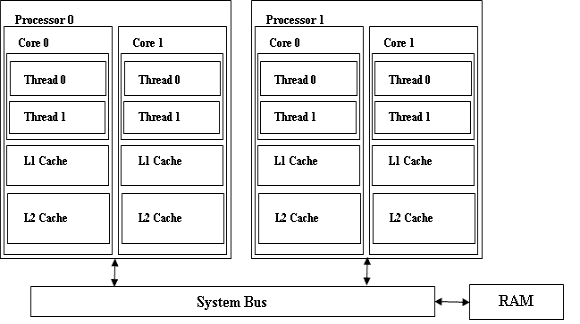
\includegraphics[scale=0.50]{background/figs/multicore_mp_system.png}}
    \caption{A typical chip multithreaded, multi-core, multiprocessor system}
    \label{fig:multicore}
\end{figure}

With the ever-growing demand of computation power, a large amount of such 
processors are grouped close together into a computer cluster with high speed 
interconnection system to further scale the system. All the cores belonging to 
the same node in the cluster shares the resources (memory system, last-level 
cache etc.) whereas cross-node resources are private to their respective nodes.  
This essentially segregates the memory system into various regions not directly 
accessible to all the cores. Accessing remote contents is possible by sending 
them as message to the requesting node which implies that accessing to different 
memory regions incurs distinct latency.  This offloads the task of ensuring the 
performance of the program to the programmer because careless handling of the 
physical location and topology of the nodes can easily saturate the 
interconnection system and cause different processors to have imbalanced 
accessing time to the same data.

Since the dawn of the artificial intelligence, GPU, due to its immense data 
parallelism capability, has seen a transformation from a peripheral device used 
in niche domains to a general-purpose mass adoption. Along with the 
re-configurability of FPGAs and domain-specific ASICs, heterogeneous systems 
contribute to a significant portion of computation power on some modern parallel 
systems. As external devices, to be able to exploit their parallelism, data has 
to be transferred from the CPU to the device and vice versa in the face of any 
synchronization or communication. 

\section{Parallel Programming Models}
\label{sec:ppm}
Parallel programming models can roughly be categorized into two class: one for 
shared-memory system and the other for distributed-memory system. The 
classification is due to the distinct ways these models deal with the 
underlying memory system.

\subsection{Shared-Memory Programming Model}
OpenMP~\cite{openmp, OpenMP4.0} is a standard programming model on a 
shared-memory system. It is an application programming interface (API) that 
supports shared memory multiprocessing programming in C, C++, and FORTRAN.

OpenMP uses a fork-join model for its parallel executions as seen in 
Figure~\ref{fig:fork-join}.
All OpenMP programs begin as a single process: the master thread. The master 
thread executes sequentially until the first parallel region construct is 
encountered. The master thread then creates a team of parallel threads.
The statements in the program that are enclosed by the parallel region construct 
are then executed in parallel among the various team threads. When the team 
threads complete the statements in the parallel region construct, they 
synchronize and terminate, leaving only the master thread~\cite{llnl_openmp}.
\begin{figure}[H]
    \centerline{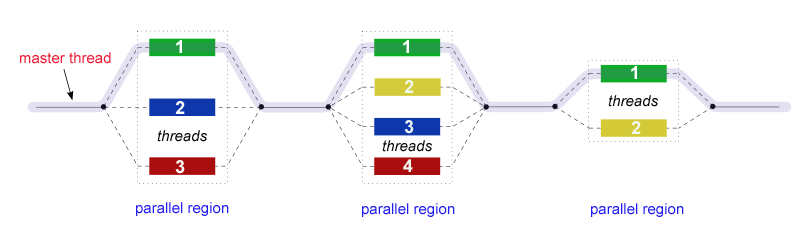
\includegraphics[scale=0.50]{background/figs/fork_join.png}}
    \caption{OpenMP uses a fork-join model}
    \label{fig:fork-join}
\end{figure}

\subsection{Task-based Parallel Programming Model}
A fork-join model creates parallel regions each of which is dedicated to solving 
a specific problem whereas the program logic is executed in sequential on the 
master thread. It introduces inefficiencies because the parallel regions can be 
far between and the sequential execution in-between keeps all the other threads 
idle. 

Task-based parallel programming model sets off to tackle this problem. In a 
task-based approach the problem is ideally re-factorized and decomposed into 
smaller functions called tasks that have clear set of inputs and outputs from 
which data dependencies can be derived unambiguously. Therefore, tasks can be 
launched and executed in parallel as long as they don't have data dependencies 
among each other and hardware resources are available. A dedicated runtime 
system is in charge of building the dependency graph and orchestrating the task 
scheduling. There are many task-based parallel programming models, the most 
prominent of which includes the OpenMP 4.0~\cite{OpenMP4.0}, Clik++~\cite{clik},
TBB~\cite{tbb} and OmpSs~\cite{ompss}.

\subsection{Distributed-Memory Programming Model}
MPI (Message Passing Interface) is a library specification for message-passing, 
proposed as a standard by a broadly based committee of vendors, implementors, 
and users. It primarily addresses the message-passing parallel programming 
model: data is moved from the address space of one process to that of another 
process through cooperative operations on each process~\cite{llnl_mpi}.

The MPI interface is meant to provide essential virtual topology, 
synchronization, and communication functionality between a set of processes 
(that have been mapped to nodes/servers/computer instances) in a 
language-independent way, with language-specific syntax (bindings), plus a few 
language-specific features. MPI programs always work with processes, but 
programmers commonly refer to the processes as processors. 

MPI library functions include, but are not limited to, point-to-point 
rendezvous-type send/receive operations, choosing between a Cartesian or 
graph-like logical process topology, exchanging data between process pairs 
(send/receive operations), combining partial results of computations (gather and 
reduce operations), synchronizing nodes (barrier operation) as well as obtaining 
network-related information such as the number of processes in the computing 
session, current processor identity that a process is mapped to, neighboring 
processes accessible in a logical topology, and so on. Point-to-point operations 
come in synchronous, asynchronous, buffered, and ready forms, to allow both 
relatively stronger and weaker semantics for the synchronization aspects of a 
rendezvous-send~\cite{wiki_mpi}.

\section{Numerical Solvers For Systems of Linear Equations}
\label{sec:solvers}

\subsection{Direct Solvers}
\subsection{Iterative Solvers}

\section{Deep Neural Networks and Their Parallelization}
\label{sec:dnn}
\subsection{Supervised Deep Learning}
\subsection{Data Parallelism}
\subsection{Model Parallelism}
